%TODO: ARREGLAR EJERCICIO 1B
\documentclass{article}
\usepackage[utf8]{inputenc}
\usepackage[spanish]{babel}
\usepackage{graphicx, graphics, float, hyperref}
\usepackage{listings}
\usepackage[a4paper, total={6in, 10in}]{geometry}

\title{SSO Práctica 1 Sesión 5}
\author{Andrés Merlo Trujillo}
\date{}
\hypersetup{
    colorlinks=true,
    linkcolor=black,
}

\begin{document}

\maketitle

\tableofcontents

\newpage
%\addcontentsline{toc}{section}{Ejercicio 1}
%\section*{Ejercicio 1}
%\begin{figure}[H]
%    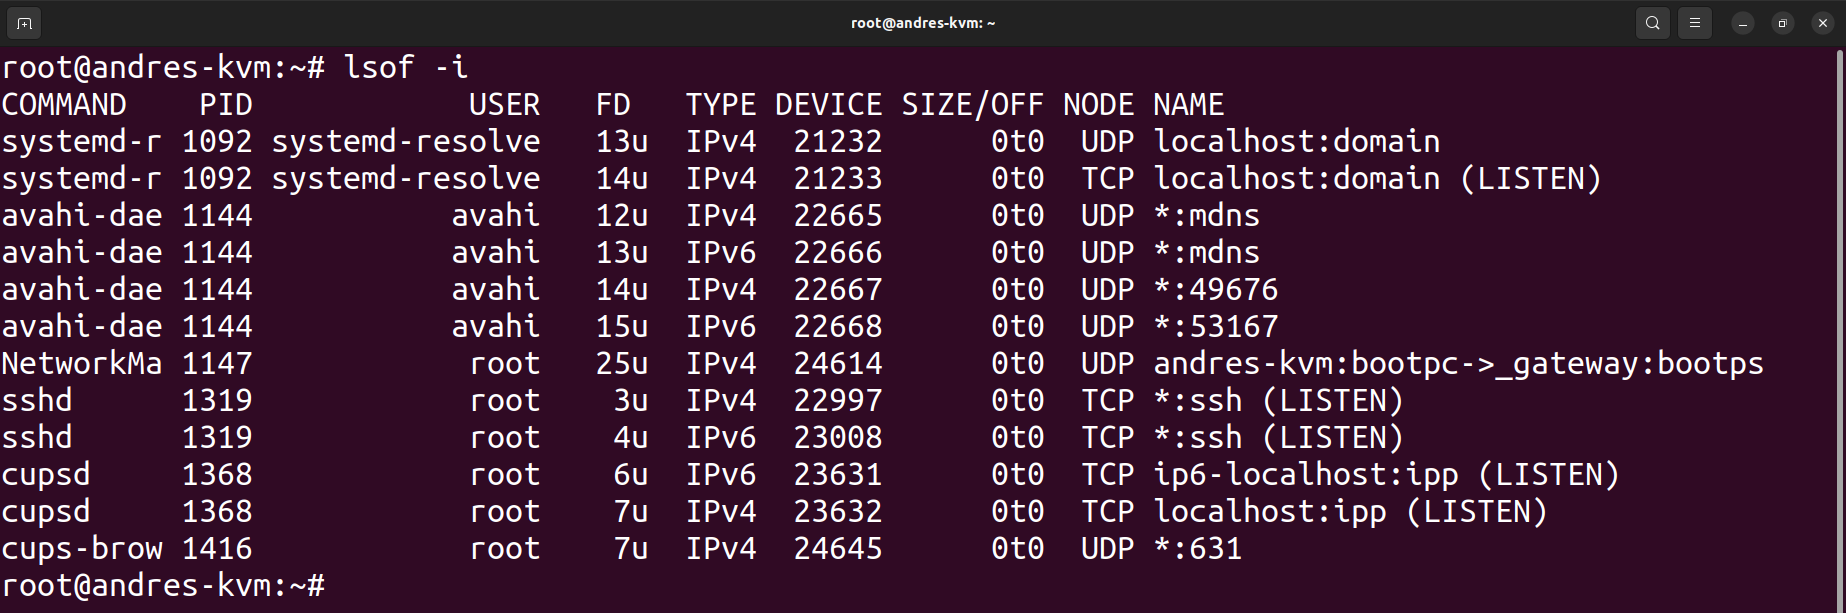
\includegraphics[width=\textwidth]{imagenes/lsofi.png}
%\end{figure}

%\addcontentsline{toc}{section}{Ejercicio 1}
%\section*{Ejercicio 1}

\addcontentsline{toc}{section}{Ejercicio 1}
\section*{Ejercicio 1}

Lo primero que hay que hacer es encriptar el pendrive, esto se puede hacer ejecutando la orden \verb|cryptsetup luksFormat /dev/device| (en mi caso es \verb|/dev/sda|, ya que estoy en una máquina virtual con un pendrive pasado por passthrough). Es importante recordar que el dispositivo no debe estar montado en ningun sitio, si lo estuviera con la orden \verb|umount punto_montaje| se desmonta.

%foto de la salida

Como se puede ver, pide una contraseña de cifrado para encriptar el dispositivo. Una vez encriptado, es necesario abrirlo, se puede hacer con la orden \verb|cryptsetup open /dev/device nombre|, donde nombre indica el nombre que se le pondrá al ser abierto (para acceder a él es necesario buscarlo en la ruta \verb|/dev/mapper/nombre|):

%Foto del comando

Una vez abierto, es necesario crear un sistema de archivos para que se pueda trabajar con él. Esto se puede hacer con la orden \verb|mkfs.ext4 /dev/mapper/device|:

%foto de la creacion

Y ahora, se puede usar la orden \verb|mount /dev/mapper/device punto_montaje| como cualquier otro dispositivo.

%foto del mount


Ahora voy a crear el siguiente archivo con algo de texto en su interior:

%foto del nano

A contuinuacion, es necesario desmontar el sistema de archivos primero y luego cerrar lam particion cifrada. Esto primero se puede hacer con la orden \verb|umoun punto_montaje|.

%FOTO DE UMOUNT

Lo siguiente es cerrar la particion encriptada, esto se realiza ejecutando la orden \verb|cryptsetup close /dev/mapper/device|

%foto de close

Este ultimo paso es opcional, ya que es imposible que se pueda escribir nada en el dispotivos estando desmontado, pero se puede ejecutar la orden \verb|eject /dev/sda| o hacerlo desde el entorno de escritorio para expulsar el dispositivo.

%foto eject

Ahora al volverlo a conectar, GNOME pide la contraseña para desencriptar.

%foto del prompt de GNOME

Una vez desencriptado, GNOME lo monta de manera automática, haciendo accesible el contenido del pendrive.

%foto del contenido

%foto del nano

Todo esto se podria haber hecho de manera manual mediante terminal realizando los comandos anteriormente mencionados en este orden:

\begin{enumerate}
    \item \verb|cryptsetup open /dev/sda sdaOpen|
    \item \verb|mount /dev/mapper/sdaOpen /mnt|
\end{enumerate}

Sin embargo, para el usuario promedio es mejor realizarlo de manera gráfica, como lo que ofrecen entornos de escritorio como GNOME o KDE.

\addcontentsline{toc}{section}{Ejercicio 2}
\section*{Ejercicio 2}

Para instalar ``Steghide'' en Ubuntu es necesario usar la orden \verb|sudo apt install steghide|

Voy a usar la siguiente imagen para ocultar un mensaje con la herramienta:

%FOTO DE LA IMAGEN DEL PAISAJE

Y voy a ocultar el siguiente mensaje:

%FOTO DEL MENSAJE

Finalmente, para ocultar el mensaje en la imagen se usa la orden \verb|steghide embed -cf imagen -ef texto|:

%SALIDA DEL COMANDO

COmo se puede observar, pide un salvoconducto, que es una contrasñé auqe hay que introducir para que se pueda extraer el contenido de la imagen.

Ahora al comparar las dos imagenes, a simple vista no hay ninguna diferencia aparente.

%COMPARACION DE LAS DOS IMAGEENES UNA AL LADO DE OTRA

Ahora, al comparar sus hashes podemos ver que son completamente distintos.

%FOTO DEL HASH

Ahora bien, existe la orden \verb|compare| que permite comparar dos imágenes y obtener el resultado en otra imagen mostrando como píxeles rojos aquellos que han sido modificados. Usando la orden \verb|compare image1 image2 -compose src diff.png| se puede obtener la siguiente imagen:

%IMAGEN DE DIFERENCIA

Como se puede ver, han sido modificados muchos pixeles de la imagen original.

Finalemtne, con la orden \verb|steghide extract -sf imagen.jpg| se puede obtener el; archivo oculto en la imagen.

%FOTO DEL COMANDO Y LA SALIDA DEL ARCHIVO COTULO

Como se puede ver, pide la contrasñea que se pedia al insertar el archivo en la imagen.


\addcontentsline{toc}{section}{Ejercicio 3}
\section*{Ejercicio 3}

Por desgracia, no he sido capaz de poder ejecutar el programa VSL de ninguna forma. He probado con Ubuntu 22.04.1 LTS y Arch Linux actualizado a día 30 de octubre de 2022 y con varias versiones de JDK (8, 11, 18 y 19) y con ninguna ha funcionado. 

Lo maximo que he conseguido ha sido que arrancase el programa, modelar el input, el decodificador y el output y elegir la imagen con el archivo oculto. Sin embargo, al darle a ejecutar experimento se produce una excepción de Java que me impide continuar.

Cabe destacar que he probado con Windows 11 también y se produce exactamente el mismo error.

%FOTO DE LA EXCEPCION DE JAVA
%Nota: El programa no he sido capaz de ejecutarlo usando Ubuntu 22.04.1 LTS. He probado con varias versiones de JDK, pero siempre saltaba con alguna excepción de Java y la ventana no se conseguia abrir. Finalemnte he optado por pasar las imagenes a otra maquina virtual que utiliza Arch Linux y en la que si puedo ejecutar el programa con OpenJDK 8.
%
%
%Primero hay que descargar el programa usando el siguiente enlace: \url{http://vsl.sourceforge.net/}.
%
%Una vez hecho esto, se descomprime y usando el comando \verb|java -jar programa.jar| se ejecuta (es necesario tener openjdk instalado).
%
%%FOTO D LA PANTALLA INICIAL
%
%Ahora hace falta conectar como aparece en el video un ``Input'', con el decodificador ``LSB.D'' y finalmente el Output. Luego, haciendo click derecho, se le da a ``Connect'' y se conectan.
%
%%foto del esquema
%
%Lo siguiente que hay que hacer, es añadirle la imagen en el input modificada, para ello, se le da click derecho y se elige la opcion ``select input''.
%
\end{document}

%\begin{figure}[H]
%    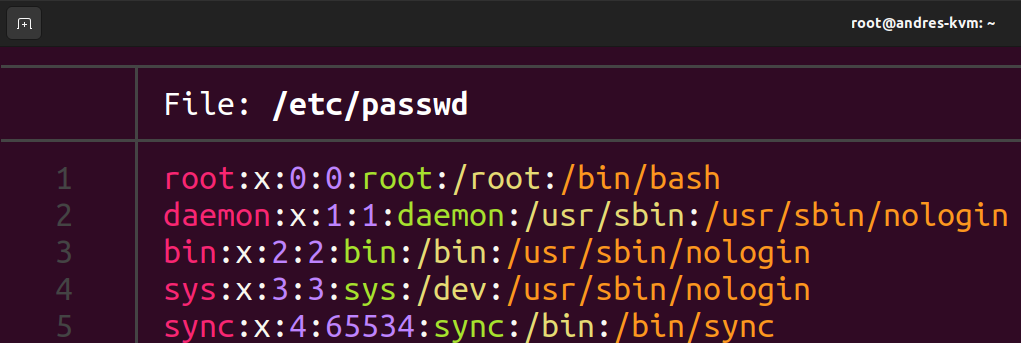
\includegraphics[width=\textwidth]{imagenes/passwdfile.png}
%    \caption{Ejemplo de entradas en el archivo.}
%\end{figure}